\documentclass{scrartcl}
\usepackage[utf8]{inputenc}
\usepackage{graphicx}
\usepackage{wrapfig}
\usepackage{listings}
\usepackage{minted}
\usepackage{subcaption}
\usepackage{csquotes}
\usepackage{hyperref}
\usepackage{amsmath}
\usepackage{biblatex}

\addbibresource{main.bib}

\title{PLSC 504: Replication Term Paper}
\subtitle{Secular Party Rule and Religious Violence in Pakistan}
\author{Mario Belledonne}
\date{\today}

\begin{document}

\maketitle

\section{Introduction}

Do terrorists cause violence in response to secular incumbency or does secular incumbency occur in response to terrorist violence?

The period of $1998 \rightarrow 2003$ in Pakistan offers a "natural experiment" due to a plurality of first-past-the-post elections where both Islamist and secular leaders competed for local elections.
These elections determine the Members of the National Assembly (MNA), who are responsible for implementing local policies at the behest of their constituency.
The authors claim that secular victories within a MNA district attenuate violence at the district level, possibly moderated by police infrastructure. 

\section{Design} \label{design}


The authors aim to measure the effect of secular rule (\ref{treatment}) on violence (\ref{outcome}) in democratic elections.

\paragraph{Data} \label{data}

The authors used reports from the BFRS Political Violence in Pakistan Dataset. This dataset tallied reports of political violence from a daily English-language newspaper, \textit{Dawn}. The geo-political units of these reports are in terms of administrative districts. This immediately posses a challenge to identification since administrative units do not correspond in a one-to-one fashion to constituencies and have re-organized over time.

The authors define a novel geo-political unit of analysis to overcome the discrepancy between districts and constituencies: the \textit{joined-district}. 
This is defined as:
\begin{displayquote}
  ...the smallest amalgamation of districts that encompasses complete MNA constituencies. 
\end{displayquote}


\paragraph{The Outcome Variable} \label{outcome}


The authors use a variety of outcomes for religious violence for a particular joined-district $i$ at election $t$, $Y_{i,t}$.

\begin{enumerate}
\item Any Event: A binary variable that is \textit{True} if any form of religious violence occured during the MNA's time in office for that district
\item Any Killed: Similar to \textit{Any Event} but referring to any deaths
\item Event Count: The number of religious-violent events
\item Number Killed: The number of deaths caused by religious violence
\item Number of days: The number of days in which at least one instance of religious violence occured.
\end{enumerate}


\paragraph{Treatment} \label{treatment}

The authors define treatment as
\begin{displayquote}
... the proportion of joined-district MNA seats
  won by secular party candidates ...
\end{displayquote}



\subsection{Instrumental Variable Identification} \label{id}

\paragraph{Difference in Means}

\begin{figure}[h]
  \centering
  \scalebox{0.5}{
    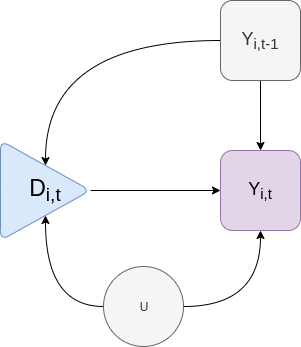
\includegraphics{replication/output/dags-ate_dim.png}
  }
  \caption{DIM Bias}
  \label{fig:ate_dim}
\end{figure}

The bivariate Difference in Means (DIM) estimator for the ATE takes the following form: 
\begin{equation} \label{eq:1}
  Y_{i,t} = \alpha + \beta * D_{i,t} + \epsilon_{i,t}
\end{equation}
Where, $D_{i,t}$ is the treatment and $\epsilon_{i,t}$ describes error.

The authors describe two potential sources of bias for DIM \ref{fig:ate_dim}:

\begin{enumerate}
\item Reverse causality/ interference: Does previous violence effect the current election?
\item Unobserved confounders between treatment and outcome.
\end{enumerate}

\paragraph{Instrumental Variables} \label{iv}

The authors resort to Instrumental Variables (IV) in order to isolate exogenous variance in treatment (cite IV).
The authors postulate that races where the secular candidate wins by a narrow margin ($\leq 3 \%$), $Z_{i,t}$, identifies an as-if random assignment for treatment,($D_{i,t}$).
In addition, the authors cite a potential backdoor for the instrument, the proportion of close races either won or lost by secular canditates by a close margin, $X_{i,t}$.
By controlling for $X_{i,t}$, the authors hope to ensure the exogeneity of the instrument.

An IV design follows five assuptions:

\begin{enumerate}
\item{Non-zero first stage: $D_{i,t} \not\!\perp\!\!\!\perp Z_{i,t}$}
\item{Exclusion Restriction: $Y_{i,t} \perp Z_{i,t} \| D_{i,t}$}
\item{Exogenous instrument}
\item{Monotonicity}
\item{Non-interference}
\end{enumerate}

The authors defend the non-zero first stage in table \ref{table:first_stage} by calculated the first-stage regression, eq \ref{eq:1}.
Given the relationship between covariate $X_{i,t}$, the proportion of close races, and the instrument, the proportion of close races that secularists win, the authors claim that the exclusion restriction holds as the only logical path that $Z_{i,t}$ could effect religious violence in a joined-district must be the proportion of seats won by secular candidates.
The authors rigorously defend the exogeneity of the instrument by ensuring that the instrument did not predict a variety of pre-treatment covariates including state capacity, agricultural production, census data (education, utilities), and voter participation. These results are replicated in \ref{exo}

While the original work does not explicitly mentioned the assumption of monotonicity, the presence of defiers would be nearly impossible.
For defiers to be present, a joined-district would have to nominate a losing candidate.
This is incredibly illogical in an adversarial, first-past-the-post system.
However, the authors note that corruption at the ballot counting office may lead to a just barely winning secularist candidate to nominated.
To this end, the authors calculate a density test on the instrument (figure \ref{fig:density}).

The Non-interference assumption is defended by a combination of lagged predictions in defending exogeneity \ref{exo} and the inclusion of the proportion of close races, $X_{i,t}$, and province-level fixed effects $\theta_p$.

\paragraph{Fixed Effects}
The original compilers (cite) of the BFRS dataset recommend using province level fixed effects, $\theta_p$ in order to control for regional differences in reporting behavior.
However, the authors note that excluding FE did not change the main estimates. (TODO add figure in results)


\begin{figure}[h]
  \centering
  \scalebox{0.5}{
    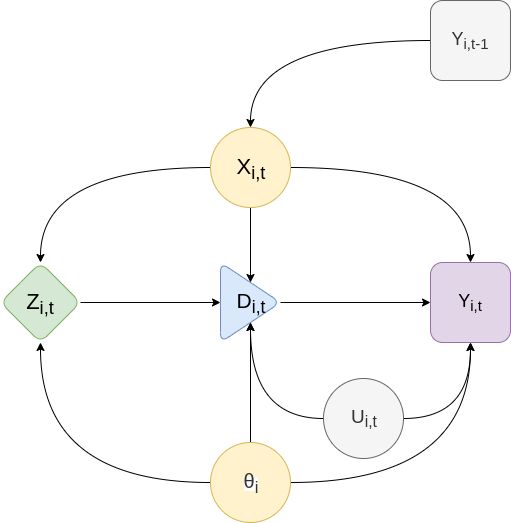
\includegraphics{replication/output/dags-ate_iv.png}
  }
  \caption{IV Model}
  \label{fig:ate_iv}
\end{figure}

In sum, figure \ref{fig:ate_iv} illustrates the model identifying the ATE.

\paragraph{2SLS Estimation}

Thus they define a two stage estimation strategy as follows:


\begin{equation} \label{eq:2}
  \widehat{D_{i,t}} = \mu + \lambda * Z_{i,t} + \kappa*X_{i,t} + \theta_p + v_{i,t}
\end{equation}

 \begin{equation} \label{eq:3}
  Y_{i,t} = \alpha + \beta * \widehat{D_{i,t}} + \gamma*X_{i,t} + \theta_{p} + \epsilon_{i,t}
\end{equation}

Where

\begin{itemize}
\item $Z_{i,t}$ describes the proportion of MNA seats won by secular candidates when in close competition with Islamist candidates (within $\pm 3\%$).
\item $\widehat{D_{i,t}}$ is the predicted proportion of MNA seats won by secular candidates across all races in that district.
\item $\theta_p$ describes a geo-spatial fixed effect of violence reporting at the province level. 
\end{itemize}

Here \ref{eq:2} refers to the first stage and \ref{eq:3} refers to the estimator of the \texttt{ATE} localized to close races between secular and Islamist MNA elections.  

\paragraph{Clustered Standard Errors}

To capture the time varying geographic nature of administrative districts, the authors included a second unit, the \textit{cluster district} that is define as follows:

\begin{displayquote}
  the smallest amalgamation of districts that contain complete MNA constituencies that did not geographically change from $1998 - 2013$.
\end{displayquote}

These cluster districts where used in calculating clustered standard errors.


\section{Results}

\subsection{Design Checks}

\paragraph{Non-zero First Stage}

\begin{table}[ht]
  \begin{center}
    \scalebox{0.85}{
      
\begin{tabular}{l c }
\hline
 & Prop. Secular Win \\
\hline
Prop. Secular Close Win  & $0.903^{***}$ \\
                         & $(0.123)$     \\
Prop. Secular Close Race & $-0.098$      \\
                         & $(0.103)$     \\
\hline
Num. obs.                & 437           \\
F statistic              & 54.446        \\
RMSE                     & 0.346         \\
\hline
\multicolumn{2}{l}{\scriptsize{\parbox{.4\linewidth}{\vspace{2pt}$^{***}p<0.01$, $^{**}p<0.05$, $^*p<0.1$. \\
       Robust SEs clustered by cluster-district area, in brackets\\ F-statistic reported for Prop.Secular Close Win}}}
\end{tabular}

    }
    \caption{First Stage Regression}
    \label{table:first_stage}
  \end{center}
\end{table}

A key component to an IV design is a non-zero first stage \ref{iv}. In other words, the exogenous instrument, $Z_{i,t}$ must have a statistically significant effect on treatment, $D_{i,t}$.
Table \ref{table:first_stage} replicates the original work where the proportion of close wins by secular candidates has a strong effect on the proportion of secular wins by any margin (eq \ref{eq:2}).

%% TODO: Explore validation of exclusion restriction
%% \paragraph{Exclusion Restriction}
%% \begin{table}[ht]
%%   \begin{center}
%%     \scalebox{0.725}{
%%       
\begin{tabular}{l c c c c c }
\hline
 & Any Event & Event Count & Any Killed & Number Killed & Number Days \\
\hline
Prop. Secular Close Win  & $-0.277$  & $12.539$  & $0.542$   & $15.823$  & $14.303^{*}$ \\
                         & $(0.684)$ & $(7.510)$ & $(0.967)$ & $(9.684)$ & $(7.984)$    \\
Prop. Secular Close Race & $-0.091$  & $-8.508$  & $-0.519$  & $-10.388$ & $-9.450^{*}$ \\
                         & $(0.386)$ & $(5.111)$ & $(0.585)$ & $(6.631)$ & $(5.502)$    \\
\hline
Num. obs.                & 437       & 437       & 437       & 437       & 437          \\
F statistic              & 9.455     & 15.030    & 4.264     & 2.639     & 14.971       \\
RMSE                     & 0.270     & 2.758     & 0.354     & 3.277     & 2.908        \\
\hline
\multicolumn{6}{l}{\scriptsize{\parbox{.4\linewidth}{\vspace{2pt}$^{***}p<0.01$, $^{**}p<0.05$, $^*p<0.1$. \\
       Robust SEs clustered by cluster-district area, in brackets\\ F-statistic reported for Prop. Secular Close Win}}}
\end{tabular}

%%     }
%%     \caption{Exclusion Restriction}
%%     \label{table:exclusion_restriction}
%%   \end{center}
%% \end{table}

\paragraph{Exogenous Instrument} \label{exo}
\begin{table}[ht]
  \begin{center}
    \scalebox{0.75}{
      
\begin{tabular}{l c c c c c }
\hline
 & Any Event & Event Count & Any Killed & Number Killed & Number Days \\
\hline
Prop. Secular Win        & $-0.066$      & $-1.165$  & $-0.127$     & $-1.404$  & $-1.162$  \\
                         & $(0.251)$     & $(1.947)$ & $(0.245)$    & $(1.969)$ & $(1.947)$ \\
Prop. Secular Close Race & $-0.364^{**}$ & $-1.802$  & $-0.313^{*}$ & $-1.696$  & $-1.811$  \\
                         & $(0.163)$     & $(1.335)$ & $(0.168)$    & $(1.398)$ & $(1.335)$ \\
\hline
Num. obs.                & 437           & 437       & 437          & 437       & 437       \\
RMSE                     & 0.301         & 2.535     & 0.355        & 2.904     & 2.540     \\
\hline
\multicolumn{6}{l}{\scriptsize{\parbox{.4\linewidth}{\vspace{2pt}$^{***}p<0.01$, $^{**}p<0.05$, $^*p<0.1$. \\
       Robust SEs clustered by cluster-district area, in brackets}}}
\end{tabular}

    }
    \caption{Placebo Check — Can Secular Victory in Close Elections at Time t Predict Prior Violence}
    \label{table:placebo}
  \end{center}
\end{table}
\begin{table}[ht]
  \begin{center}
    \scalebox{0.75}{
      
\begin{tabular}{l c c c }
\hline
 & No Fixed Effects & Disctrict Cluster FE & Disctrict Cluster + Province-Year FEs \\
\hline
Secularist Close Race & $-0.355^{***}$ & $-0.386^{***}$ & $-0.257^{***}$ \\
                      & $(0.119)$      & $(0.111)$      & $(0.091)$      \\
\hline
Num. obs.             & 437            & 437            & 437            \\
RMSE                  & 0.371          & 0.337          & 0.294          \\
\hline
\multicolumn{4}{l}{\scriptsize{\parbox{.4\linewidth}{\vspace{2pt}$^{***}p<0.01$, $^{**}p<0.05$, $^*p<0.1$. \\
       Robust SEs clustered by cluster-district area, in brackets}}}
\end{tabular}

    }
    \caption{Correlation Between Close Secular/Nonsecular Elections and Violence at Time t-1}
    \label{table:4}
  \end{center}
\end{table}

In order to address the potential influence of reverse causality, the authors attempted to predict the previous outcome for a given joined-district $Y_{i,t-1}$.
I was able to reproduce the authors' null result \ref{table:placebo}.
However, it is important to note that the instrument can predict $Y_{i,t-1}$.
The authors explore this correlation in \ref{table:4}, showing that close secular races tend to occur in low violence joined-districts.
Further analysis, shows that the instrument does not predict a variety of pre-treatment covariates such as agricultural production, education, and civil infastructure. (TODO)

\paragraph{Monotonicity}

\begin{figure}[h]
  \centering
  \scalebox{0.5}{
    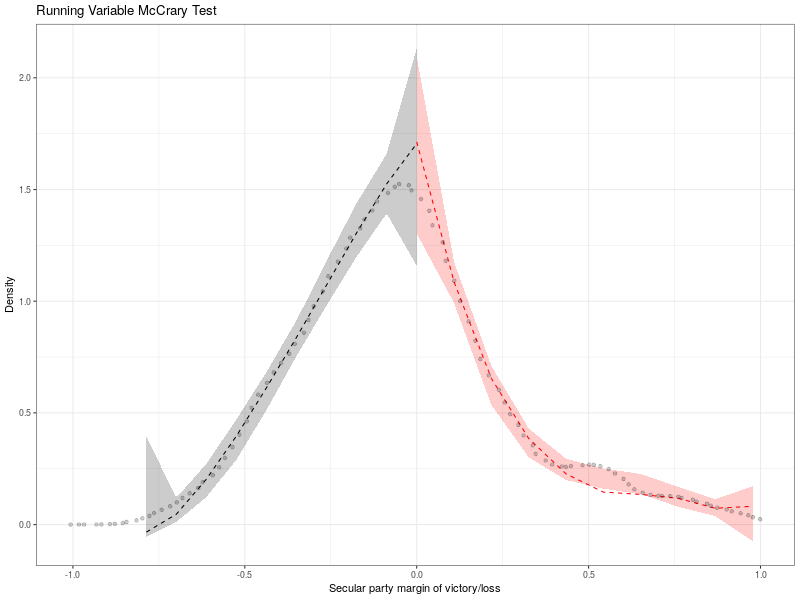
\includegraphics{replication/output/fig_a4.png}
  }
  \caption{McCrary Density Test}
  \label{fig:density}
\end{figure}
%% TODO: Add mccrary test table

In an effort to obviate concerns of sorting described in \ref{iv}, the authors perform a density test that shows a null result (fig \ref{fig:density}).
While this cannot conclusively rule out sorting or attrition, a null result suggests that treatment is as good as random under the instrument (TODO: cite McCrary). 

\subsection{Main Effect}

\paragraph{IV Estimates of ATE} \label{ate:iv}

\begin{table}[ht]
  \begin{center}
    \scalebox{0.75}{
      
\begin{tabular}{l c c c c c }
\hline
 & Any Event & Event Count & Any Killed & Number Killed & Number Days \\
\hline
Prop. Secular Win        & $-0.660^{***}$ & $-4.654^{**}$ & $-0.477^{*}$ & $-3.266$  & $-4.700^{**}$ \\
                         & $(0.215)$      & $(1.744)$     & $(0.275)$    & $(2.144)$ & $(1.767)$     \\
Prop. Secular Close Race & $0.031$        & $0.837$       & $0.004$      & $0.281$   & $0.947$       \\
                         & $(0.085)$      & $(0.875)$     & $(0.161)$    & $(1.276)$ & $(0.884)$     \\
\hline
Num. obs.                & 437            & 437           & 437          & 437       & 437           \\
F statistic              & 9.831          & 11.564        & 4.500        & 2.597     & 10.839        \\
RMSE                     & 0.357          & 3.025         & 0.389        & 3.194     & 3.114         \\
\hline
\multicolumn{6}{l}{\scriptsize{\parbox{.4\linewidth}{\vspace{2pt}$^{***}p<0.01$, $^{**}p<0.05$, $^*p<0.1$. \\
       Robust SEs clustered by cluster-district area, in brackets\\ F-statistic reported for Prop. Secular Win}}}
\end{tabular}

    }
    \caption{Instrumental Variable Results}
    \label{table:2}
  \end{center}
\end{table}

In table \ref{table:2}, we replicate the main estimate, the ATE of the proportional of seats won by secular leaders on religious violence across joined-districts and time. 

\begin{table}[ht]
  \begin{center}
    \scalebox{0.75}{
      
\begin{tabular}{l c c c c c }
\hline
 & Any Event & Event Count & Any Killed & Number Killed & Number Days \\
\hline
Prop. Secular Win        & $-0.660^{**}$ & $-4.654^{**}$ & $-0.477$  & $-3.266$  & $-4.700^{**}$ \\
                         & $(0.229)$     & $(1.866)$     & $(0.296)$ & $(2.309)$ & $(1.892)$     \\
Prop. Secular Clost Race & $0.031$       & $0.837$       & $0.004$   & $0.281$   & $0.947$       \\
                         & $(0.086)$     & $(0.907)$     & $(0.173)$ & $(1.362)$ & $(0.916)$     \\
\hline
R$^2$                    & -0.580        & -0.486        & -0.164    & -0.169    & -0.482        \\
Adj. R$^2$               & -0.602        & -0.507        & -0.180    & -0.185    & -0.503        \\
Num. obs.                & 437           & 437           & 437       & 437       & 437           \\
RMSE                     & 0.357         & 3.025         & 0.389     & 3.194     & 3.114         \\
\hline
\multicolumn{6}{l}{\scriptsize{Robust SEs clustered by cluster-district area, in brackets}}
\end{tabular}

    }
    \caption{IV with CR2 SE estimation}
    \label{table:2_cr2}
  \end{center}
\end{table}

However, it is important to note that the significance of these estimates are sensitive to the standard error estimation strategy (\texttt{stata}).
In table \ref{table:2_cr2}, I recalculated the effects using \texttt{CR2} standard error estimation and the effect for \textit{Any Killed} was no longer significant.

\paragraph{DIM estimates of ATE}

\begin{table}[ht]
  \begin{center}
    \scalebox{0.75}{
      
\begin{tabular}{l c c c c c }
\hline
 & Any Event & Event Count & Any Killed & Number Killed & Number Days \\
\hline
Secularist Close Win & $-0.176$           & $-1.265$           & $-0.141$           & $-0.769$           & $-1.265$           \\
                     & $[-0.373;\ 0.020]$ & $[-2.654;\ 0.123]$ & $[-0.331;\ 0.049]$ & $[-2.142;\ 0.605]$ & $[-2.654;\ 0.123]$ \\
\hline
R$^2$                & 0.330              & 0.393              & 0.398              & 0.390              & 0.393              \\
Adj. R$^2$           & 0.267              & 0.336              & 0.341              & 0.332              & 0.336              \\
Num. obs.            & 59                 & 59                 & 59                 & 59                 & 59                 \\
RMSE                 & 0.279              & 2.303              & 0.280              & 2.435              & 2.304              \\
\hline
\multicolumn{6}{l}{\scriptsize{Robust SEs clustered by cluster-district area, in brackets}}
\end{tabular}

    }
    \caption{Difference in Means Estimate}
    \label{table:3}
  \end{center}
\end{table}

In an effort to appeal to the strength of their data and design, the authors attempt to estimate the \texttt{ATE} using the difference-in-means estimator (table \ref{table:3}).
To this end, the authors restrict the dataset to 59 years and joined-district points where there was a single close election between secular and Islamist candidates. I was able to replicate the original findings, with a significant negative effect for \textit{Any Event, Event Count} and \textit{Number of Days}.


\begin{table}[ht]
  \begin{center}
    \scalebox{0.75}{
      
\begin{tabular}{l c c c c c }
\hline
 & Any Event & Event Count & Any Killed & Number Killed & Number Days \\
\hline
Secularist Close Win & $-0.176^{*}$ & $-1.265^{*}$ & $-0.141$  & $-0.769$  & $-1.265^{*}$ \\
                     & $(0.095)$    & $(0.670)$    & $(0.092)$ & $(0.663)$ & $(0.670)$    \\
\hline
R$^2$                & 0.330        & 0.393        & 0.398     & 0.390     & 0.393        \\
Adj. R$^2$           & 0.267        & 0.336        & 0.341     & 0.332     & 0.336        \\
Num. obs.            & 59           & 59           & 59        & 59        & 59           \\
RMSE                 & 0.279        & 2.303        & 0.280     & 2.435     & 2.304        \\
\hline
\multicolumn{6}{l}{\scriptsize{Robust SEs clustered by cluster-district area, in brackets}}
\end{tabular}

    }
    \caption{DIM ATE with CR2 SE Estimation}
    \label{table:3_cr2}
  \end{center}
\end{table}

Table \ref{table:3_cr2} shows the results calculated with \texttt{CR2} standard errors. 

It is important to note that while the DIM estimates are significant, the authors previously described confounders (\ref{fig:ate_dim}) that would bias the DIM estimate (cite?).
In particular, without $X_{i,t}$, geographic or time-varying interference may be present.
Figure (TODO) shows that the IV and DIM estimates for the ATE do indeed significantly differ. 


\subsection{Mechanisms}

The later section of the source, the authors perform explanatory analysis to illustrate potential mechanisms of secular MNA seats on religious violence. One explored avenue was the electoral accountability. The authors claim that secular leaders often include diminished religious violence as a campaign promise. The authors then predict that secular MNA candidates expect to suffer in future elections if religious violence does occur during their tenure. 

To test their prediction, the authors estimate the causal effect of religious violence in the previous term on the proportion of secular MNA seats in the following election.
I was able to reproduce these estimates in full (table \ref{table:mechanisms})

\begin{table}[ht]
  \begin{center}
    \scalebox{0.75}{
      
\begin{tabular}{l c c c c }
\hline
 &  &  &  &  \\
\hline
OLS                                          &                &                &               &               \\
                                             &                &                &               &               \\
\quad Prop. Secular (t-1) x Any violence     & $-0.115^{***}$ &                & $-0.102^{**}$ &               \\
                                             & $(0.040)$      &                & $(0.043)$     &               \\
\quad Prop. Secular (t-1) x Event count (ln) &                & $-0.018^{***}$ &               & $-0.014^{*}$  \\
                                             &                & $(0.006)$      &               & $(0.007)$     \\
\quad Any violence                           & $0.105^{***}$  &                & $0.086^{***}$ &               \\
                                             & $(0.028)$      &                & $(0.024)$     &               \\
\quad Prop. secularist wins (t - 1)          & $0.038$        & $-0.053^{**}$  & $0.050$       & $-0.030$      \\
                                             & $(0.043)$      & $(0.026)$      & $(0.050)$     & $(0.031)$     \\
Event count                                  &                & $0.018^{***}$  &               & $0.015^{***}$ \\
                                             &                & $(0.004)$      &               & $(0.004)$     \\
\hline
Num. obs.                                    & 344            & 344            & 344           & 344           \\
RMSE                                         & 0.139          & 0.138          & 0.126         & 0.127         \\
\hline
\multicolumn{5}{l}{\scriptsize{\parbox{.4\linewidth}{\vspace{2pt}$^{***}p<0.01$, $^{**}p<0.05$, $^*p<0.1$. \\
       Robust SEs clustered by cluster-district area, in brackets \\ Province Fixed effects omitted}}}
\end{tabular}

    }
    \caption{Mechanisms - Electoral Incentives}
    \label{table:mechanisms}
  \end{center}
\end{table}

\section{Discussion}


\section{Future work}
\subsection{Mechanisms of Main Effect}

The authors illustrate potential mechanisms for their main finding (the reduction of religious violence due to secular victories). These include electoral incentives (in terms of voter accountability if religious violence does arise in the presence of a secular district), politician characteristics, state capacity (concentration of police force in secular districts).

\section{Conclusion}


\end{document}
